% SPDX-License-Identifier: Apache-2.0
\documentclass[11pt,letterpaper]{article}
\usepackage[T1]{fontenc}
\usepackage[utf8]{inputenc}
\usepackage{lmodern,microtype}
\usepackage[margin=0.86in,headheight=16pt]{geometry}
\usepackage{amsmath,amssymb,graphicx,booktabs,tabularx,array,longtable}
\usepackage{xcolor,enumitem,fancyhdr,titlesec,caption,float,placeins}
\usepackage[most]{tcolorbox}
\usepackage[numbers,sort&compress]{natbib}
\usepackage{xurl}
\usepackage{catchfile}
\CatchFileDef{\NumericalRows}{numerical-table.tex}{}
\CatchFileDef{\EconomicRows}{economic-table.tex}{}
\usepackage[colorlinks=true,linkcolor=teal,citecolor=teal,urlcolor=teal]{hyperref}
\definecolor{ink}{HTML}{172D3B}
\definecolor{teal}{HTML}{006B63}
\definecolor{copper}{HTML}{A4653D}
\definecolor{mist}{HTML}{EEF6F4}
\hypersetup{pdftitle={AGI Alpha Flywheel: The Enterprise That Invents Its Next Advantage},pdfauthor={Vincent Boucher, President of MONTREAL.AI},pdfsubject={Executed specialist learning and conditional commercial expansion},pdfkeywords={Transformational intelligence, specialist learning, scheduling, enterprise economics, reproducibility}}
\setlength{\parindent}{0pt}
\setlength{\parskip}{5.5pt}
\setlength{\emergencystretch}{2em}
\setlist{topsep=4pt,itemsep=3pt,leftmargin=*}
\titleformat{\section}{\large\bfseries\color{ink}}{\thesection}{0.7em}{}
\titleformat{\subsection}{\normalsize\bfseries\color{teal}}{\thesubsection}{0.7em}{}
\captionsetup{font=small,labelfont=bf,skip=7pt}
\pagestyle{fancy}
\fancyhf{}
\fancyhead[L]{\small\color{ink}AGI ALPHA FLYWHEEL}
\fancyhead[R]{\small\color{teal}The next advantage}
\fancyfoot[L]{\scriptsize Executed numerical evidence $\cdot$ Conditional enterprise model}
\fancyfoot[R]{\small\thepage}
\renewcommand{\headrulewidth}{0.3pt}
\newtcolorbox{findingbox}{colback=mist,colframe=teal,boxrule=0.6pt,arc=1mm,left=9pt,right=9pt,top=8pt,bottom=8pt}
\newcommand{\USD}{US\$}
\newcommand{\CAD}{C\$}
\newcolumntype{L}[1]{>{\raggedright\arraybackslash}p{#1}}
\newcolumntype{Y}{>{\raggedright\arraybackslash}X}
\renewcommand{\bibfont}{\small}
\setlength{\bibsep}{3pt}
\begin{document}
\hypersetup{pageanchor=false}
\begin{titlepage}
\vspace*{0.3in}
{\small\bfseries\color{teal}MONTREAL.AI RESEARCH\hfill 27 OCTOBER 2026}\par
\vspace{0.45in}
{\Large\bfseries AGI ALPHA FLYWHEEL}\par
\vspace{0.18in}
{\fontsize{31}{35}\selectfont\bfseries\color{ink}The Enterprise That\par Invents Its Next\par Advantage}\par
\vspace{0.22in}
{\large Transformational Intelligence, Specialist Learning\par and the Creation of New Profitable Work}\par
\vspace{0.3in}
{\large\bfseries Vincent Boucher}\par
{\normalsize President of MONTREAL.AI}\par
\vspace{0.28in}
\begin{findingbox}
\textbf{An executable test of three interacting loops.}\par
Useful work produces a learned scheduling policy. Optional practice improves it. A fresh recipient reuses it. A decision-making enterprise weighs retention, sharing, additional search and a new offering against complete costs. The experiment also preserves the case where ordinary methods are the better investment.
\end{findingbox}
\vspace{0.1in}
\textbf{Evidence in this edition.} Eight productive-development cases; 24 Gym cases; 24 development cases; 80 fresh primary cases; 12 further fresh cases challenging the learned policy with more generic search; executed native journal, authentication-fixture and accounting interfaces; matched simulated enterprises; source-bound evidence and a bilingual companion.
\vfill
{\bfseries\color{teal}FIND YOUR ALPHA. BUILD YOUR SUCCESSOR $\Omega$.}\par
\vspace{0.12in}
{\small Research edition 1.0. Numerical learning is executed. Frontier-model behavior, customer demand and collections are not live observations. No achieved AGI, specialist ASI or autonomous commercial invention is claimed.}
\end{titlepage}
\hypersetup{pageanchor=true}

\begin{abstract}
Can productive experience improve both an automated enterprise's capabilities and the set of offerings it can profitably deliver? We implement a bounded test coupling manufacturing scheduling, numerical specialist development, executable transfer, existing AGI ALPHA accounting and authority interfaces, and a non-anticipating enterprise simulator. A researcher-authored cross-entropy learner develops seven dispatch parameters from eight synthetic productive jobs, then optionally practices on 24 additional problems. On 80 fresh cases, the resulting v2 reduces the nominal scheduling objective by 9.04\% relative to a matched 48-candidate generic portfolio; productive v1 already supplies a 7.71\% gain. The incremental Gym effect is 1.42\%. With the same risk evaluator and scenario budget, composed v2 reduces the robust objective by 7.81\% versus Beta, but the separately isolated contribution of scenario ranking is inconclusive. All learned schedules meet the fixed technical thresholds; Beta meets 76/80 nominal and 78/80 robust thresholds. A further twelve-case confirmation shows that tripling generic search can catch up with very little additional measured solver time. Matched enterprise simulations support conditional profitability and some selective retention, while showing that most modeled new-offering value is also available to an equally equipped Beta enterprise. Identical library and graph policies tie. The contribution is an inspectable mechanism and a decision boundary: useful learning is demonstrated within a finite computational budget, but its scientific existence does not establish commercial necessity, unique product creation, live frontier superiority or sustained compounding.
\end{abstract}

\section{The question and the answer this evidence can support}

An enterprise can improve a job without improving its business. A better dispatch rule can reduce late work, yet a buyer may already accept the original schedule. Another agent can run the rule, yet the avoided computation may cost less than admission and upkeep. A new product can generate attractive simulated profit while being equally deliverable by ordinary methods. These separations determine the experiment rather than appearing only as qualifications after a favorable result.

The central question is whether an enterprise can use productive experience to expand what it can do and what it can profitably sell, while choosing learning and investment intelligently. We make the mechanism executable in a demanding but bounded numerical domain. The beneficiary is a manufacturing planner with finite machines, releases, due dates, eligibility restrictions and setup costs. The initial deliverable is a checked schedule and its reproducible decision dossier. The adjacent deliverable adds risk-aware sequence selection under uncertain processing durations. Neither deliverable controls a physical plant.

\begin{findingbox}
\textbf{Four different findings must remain separate.}
\begin{enumerate}
\item \textbf{Production:} a competent Beta enterprise can be profitable under declared market and operating assumptions.
\item \textbf{Learning:} productive experience and optional Gym practice yield a measured, transferable numerical advantage at a fixed search budget.
\item \textbf{Program value:} retention and sharing can add conditional value, but benefits diminish with low demand, fast obsolescence, a stronger baseline and unnecessary development cost.
\item \textbf{New productive possibility:} the stronger claim that specialist composition uniquely enables the next profitable offering is \emph{not established} in this edition.
\end{enumerate}
\end{findingbox}

This is an implemented contribution, with explicit limits. The numerical learner updates an executable policy, not proprietary frontier-model weights. The enterprise is a finite decision program, not an autonomously discovered corporation. Native signatures, trust checks and accounting are actual code executions over synthetic identities and simulated amounts. Published frontier-model specifications inform operating roles and token-price assumptions, not a measured claim about those models' task performance.

\begin{figure}[htbp]
\centering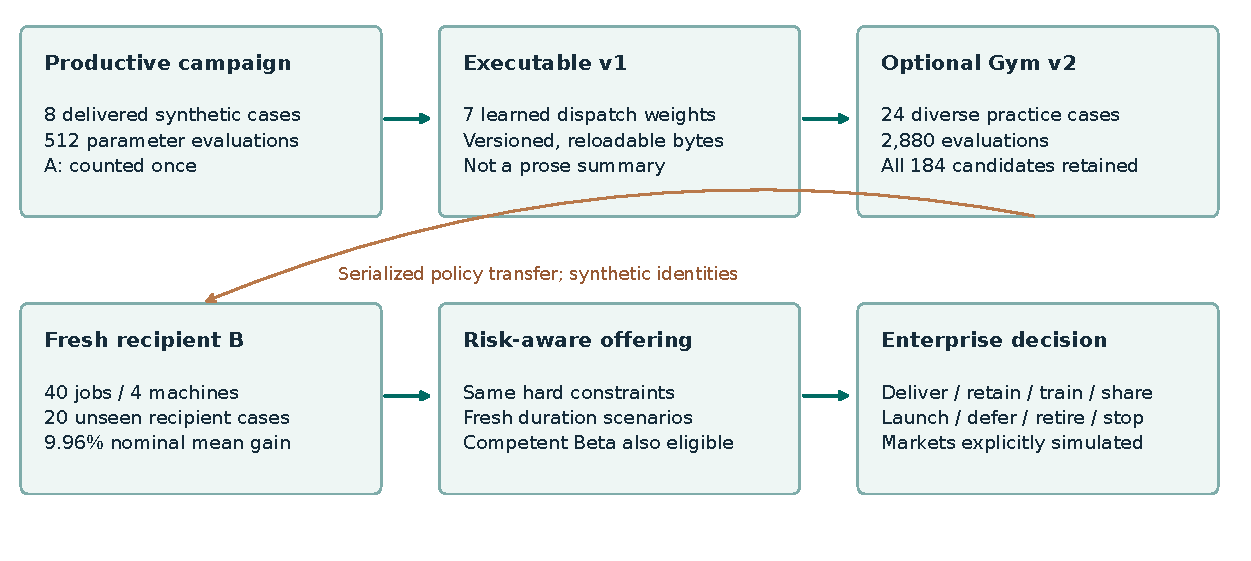
\includegraphics[width=\linewidth]{figures/productive-lineage.pdf}
\caption{The inspectable productive lineage. Every transition has an artifact and a scope. The lineage is executed as a research mechanism; an enterprise policy remains free to reject its optional stages. The eight originating jobs are synthetic engagements with saved deliverables and technical verdicts.}
\label{fig:lineage}
\end{figure}

% SPDX-License-Identifier: Apache-2.0
% Input-ready methods and related work; results belong in the parent manuscript.

\section{Research design and intellectual lineage}
\label{sec:methods-design}

The study separates three optional decisions. The \emph{production loop} accepts useful work, prices and delivers it, collects payment after acceptance, and preserves operating funds. The \emph{capability loop} retains a reusable method from delivery, optionally improves it through additional practice, and admits or retires it after assessment. The \emph{opportunity loop} asks whether available methods justify another offering. These loops can interact without becoming prerequisites for commercial success: an enterprise can remain profitable through production alone, preserve cash, reject a candidate, or stop. We investigate a finite decision system, not an inevitable trajectory toward increasing intelligence.

The inherited conceptual standard is purpose-preserving reformulation: a changed representation, experiment, or workflow must still satisfy the original beneficiary's requirements \cite{boucher2026transformational}. The existing Successor~$\Omega$ manuscript supplies a bounded construction-and-transfer precedent, including a strong conventional comparator and costs of inheritance \cite{boucher2026successor}. The unified AGI ALPHA manuscript proposes the wider institutional substrate; its architectural ambitions are not treated as demonstrated autonomous profit \cite{boucher2026unified}. We inspected these available sources and the protected-flywheel implementation at repository commit \texttt{80b345828f34fd8a6e592977dd17ef37141305f4} \cite{montrealai2026runtime}. The separately referenced original Gym/Specialist ASI document, Validated Skills Graph material, and Proof Loops material were not recovered in this source audit. We follow the supplied research requirements without claiming to have read or replicated those unavailable sources.

Algorithm portfolios motivate competent opportunity selection rather than a deliberately weak baseline \cite{xu2008satzilla}. Learning dispatch rules has demonstrated transfer within published scheduling experiments \cite{zhang2020dispatch}, and offline dispatch learning provides a precedent for extracting value from existing schedules \cite{remmerden2025offline}. Broad constraint-programming comparisons motivate an additional conventional solver challenge \cite{lan2025pyjobshop}. Such precedents do not establish our algorithm's superiority. Independent evaluation of learned optimizers also shows why training expenditure and tuning requirements cannot be omitted from an improvement claim \cite{rezk2023velo}. Our contribution is therefore an inspectable connection between numerical capability development, transfer, and conditional enterprise decisions, using established optimization machinery.

\section{The offering, preserved purpose, and independent acceptance}
\label{sec:methods-offering}

The beneficiary is a manufacturing planner with a validated batch of 32--64 nonpreemptive jobs and three or four unrelated parallel machines. The nominal offering produces machine assignments, ordered operations with start and completion times, an executable schedule, and an acceptance report. Inputs specify machine-dependent processing times, eligible machines, releases, due dates, priorities, and family-dependent setup times. The proposed commercial boundary is one facility and one planning batch; customer data preparation, objectives, and permissions must be agreed before execution. ERP integration, plant actuation, regulated engineering approval, and an operating service-level guarantee are outside this experiment. Recorded computation time is not a qualified customer turnaround time. The enterprise model allocates 0.75 capacity hours per nominal delivery and 1.6 per risk-aware delivery; these are assumptions, not observed labor or latency requirements.

For job $j$, let $r_j,d_j,w_j$ denote release, due date, and positive priority; $p_{jk}$ is its processing time on eligible machine $k$. Every job appears exactly once, starts no earlier than its release, runs without interruption for the assigned processing time, and respects predecessor-dependent setup and machine nonoverlap. The independent verifier reconstructs these obligations from the instance and delivered schedule rather than trusting the producer's reported score. With completion $C_j$, makespan $C_{\max}$, and mean processing time $\bar p$, nominal quality is
\begin{equation}
 J(S)=\frac{\sum_j w_j(C_j-d_j)_+ +0.1\bigl(\sum_jw_j\bigr)C_{\max}}
 {\bigl(\sum_jw_j\bigr)\bar p}.
 \label{eq:nominal-objective}
\end{equation}
The fixed reference is earliest-due-date ordering with earliest feasible eligible-machine completion. Nominal acceptance requires all hard constraints and $J(S)\leq0.97J(S_{\mathrm{EDD}})$. EDD defines the contractual improvement threshold; the competent Beta portfolio, described below, defines the internal Alpha comparison. Neither replaces the human-service commercial reference.

The adjacent offering supplies a duration-risk report and a schedule selected for uncertain processing times. It replays the same machine assignment and job order while propagating release, setup, and realized completion times. It does not implement rolling rescheduling, machine-breakdown recovery, or an unrestricted disruption-management service. For scenario losses $J_1,\ldots,J_N$, its objective is
\begin{equation}
 R_N(S)=\tfrac12\overline{J}+\tfrac12\operatorname{CVaR}_{0.9,N}(J),
 \label{eq:risk-objective}
\end{equation}
where the empirical tail averages sorted losses from index $\lfloor0.9N\rfloor$ onward. Acceptance requires nominal feasibility and $R_{64}(S)\leq0.95R_{64}(S_{\mathrm{EDD}})$ on identical, fresh scenarios. Sixty historical synthetic duration observations per machine estimate log-duration dispersion; selection sees those estimates, never the generator's latent dispersion. A common lognormal shock induces within-scenario correlation. Selection uses 24 scenarios and acceptance uses 64 separately seeded scenarios drawn from the latent model.

The transformation being tested is concrete. The purpose remains an executable, constraint-valid production plan. The obstacle is repeated search over dispatch priorities and vulnerability to duration variation. The alternatives are a retained dispatch policy and composition with scenario-based risk ranking. Matched fresh objectives distinguish useful improvement from easier scoring; original instance constraints remain fixed. A technically accepted artifact is commercially useful only if its complete incremental cost and buyer acceptance justify offering it. The new product menu is researcher specified; neither autonomous opportunity discovery nor a sale follows from its technical availability.

\section{Executable learning, transfer, and causal comparisons}
\label{sec:methods-learning}

The generator defines four strata: producer $(32,3)$, recipient $(40,4)$, scale $(64,4)$, and shifted $(48,3)$ job--machine dimensions. Processing heterogeneity, eligibility, releases, due-date tightness, setup families, and weights vary. Shifted cases increase eligibility restrictions, release dispersion, setup burden, and duration uncertainty. These are synthetic unfamiliar instances, not independent factories or a representative industrial benchmark collection.

The retained artifact is a seven-coordinate dispatch policy $\theta$. At each step, it scores feasible job--machine pairs using log processing time, remaining due-date slack, negative log priority, setup, release waiting, predicted tardiness, and completion time; duration-like features are normalized by $\bar p$. The lowest-scoring feasible pair is scheduled. A risk multiplier can inflate planned duration using estimated dispersion while actual schedule durations remain the supplied nominal times. Researchers authored this representation, generator, solver family, and update mechanism. The parameters themselves are learned by executed cross-entropy search, not assigned a guaranteed gain and not discovered autonomously.

For training instances $i$, define $q_i(\theta)=J_i(S_\theta)/J_i(S_{\mathrm{EDD}})$. The loss is
\begin{equation}
 L(\theta)=\operatorname{mean}_i q_i(\theta)
             +0.05\operatorname{sd}_i q_i(\theta).
\end{equation}
Cross-entropy optimization \cite{rubinstein1999crossentropy} samples clipped Gaussian coordinates in $[-3,5]^7$, evaluates complete schedules, retains the best observed policy, and updates elite statistics:
\begin{align}
 \mu_{g+1}&=0.3\mu_g+0.7\overline{\theta}_{\mathrm{elite}},\\
 \sigma_{g+1}&=\max\{0.12,\;0.3\sigma_g+0.7\operatorname{sd}(\theta_{\mathrm{elite}})\}.
\end{align}
All candidates, including unsuccessful ones, remain in the evidence. Version~v1 uses eight producer cases, four generations, population 16, and four elites: 512 schedule evaluations. This is a batch reconstruction of learning within eight simulated productive deliveries, not a claim that a live agent learned sequentially from paid customers. Version~v2 starts from v1 and optionally practices on 24 distinct producer, recipient, and scale cases, with six generations, population 20, and five elites: 2,880 additional evaluations. That extra campaign belongs to R\&D; v1's within-delivery learning is charged once within delivery.

Development uses 24 further cases, and confirmation uses 80 new cases balanced across all four strata. Learning receives only productive and Gym cases. A source-and-policy digest is written before confirmation, and serialized policies are reloaded for recipient use. This demonstrates executable transfer of parameters with their implementation, rather than transfer of a prose summary. The original interrupted run is preserved: after 24 development cases and six uninspected confirmation cases, origin-deliverable recording and latent-parameter isolation were repaired, and fresh confirmation seeds were allocated. Outcomes from the interrupted confirmation were not used for policy tuning. Holdouts are protected by program data flow and recorded procedure, not by an independent cryptographic custodian.

Every primary solve receives 48 schedule candidates. Beta has a classical dispatch portfolio, local parameter search, tool-based verification, and the same generic 24-scenario risk evaluator available to the learned policies. The \texttt{beta\_plus} diagnostic expands the classical parameter grid at the same candidate budget; it is a different allocation of finite search, not a universally stronger model. v1 adds its learned vector. v2 adds the Gym vector but deliberately removes scenario ranking in the risk-aware task. The composed policy restores that complement. Reversed learned coordinates provide a falsification control, not a competent commercial baseline. Comparisons among v1, v2, composed, Beta, and the expanded grid separate retained knowledge, additional practice, and composition. Scenario-ranking removal saves computation, so that ablation is not an equal-scenario-budget superiority claim.

Twelve prespecified confirmation cases, three per stratum, also receive OR-Tools CP-SAT optimization from both Beta and composed warm starts. Each call has one worker and 0.08 deterministic-time units, with the verified warm start retained if the solver finds no better feasible schedule. This is a separate solver-budget envelope; deterministic time is not wall-clock time or 48 dispatch candidates. It challenges whether generic optimization erases an advantage without asserting global optimality. A secondary 144-candidate Beta catch-up experiment reuses those cases and is explicitly exploratory. A separately frozen quality-frontier analysis reports every improvement threshold in $\{0,.05,.10,.15,.20,.30,.40\}$; it changes neither the primary 3\%/5\% criteria nor the primary enterprise analysis. A further separately frozen addendum uses the original 24 development cases and twelve new cases, seeds 61000--61011, for matched Beta48, learned48 and Beta144 runs with no retraining. A per-contract economic sensitivity prices the additional elapsed solver time once and sweeps additional program costs. Paired gains use case-matched bootstrap resampling; these intervals describe the finite generated task distribution.

\section{Frontier foundation and protected system boundary}
\label{sec:methods-foundation}

Official documentation was verified on 27 October 2026. The proposed general reasoning configuration is \texttt{gpt-6-astra} with high reasoning effort; visual interaction and packaging use \texttt{gpt-6.1-terra} with medium effort through the Responses API. Published standard input/output prices are respectively US\$10/50 and US\$1/5 per million tokens; both pages specify 1,050,000 context tokens and 128,000 maximum output tokens \cite{openai2026astra,openai2026terra}. Documented fine-tuning is unsupported for these models. No proprietary weights are updated. Public aliases and published access tiers were checked; account entitlement, quota, immutable dated snapshots, and realized quality were not. ChatGPT Pro is a subscription plan, not an API model identifier or automatic API access \cite{openai2026plans}.

The cost model assumes aggregate nominal-job usage of 240,000/70,000 Astra input/output tokens and 150,000/30,000 Terra tokens, with a 2.3 multiplier for the risk-aware offering. These are unmeasured orchestration budgets. Published long-context surcharges apply per request above 272,000 input tokens, while cache, speed, tool, and regional charges require separate accounting \cite{openai2026pricing}. The simulation uses standard uncached rates and explicit tool allowances; a future live run must record request lengths, retries, tools, and actual bills. Its Beta is a competent numerical portfolio proxy, not a measured ceiling on frontier reasoning with tools, experiments, and revision. Expanded-grid controls, actual 144-candidate compute expansion and a hypothetical best-capability Beta envelope are kept separate. The first two are computational diagnostics; the last is an explicitly modeled future-catch-up bound. None measures a successor frontier model.

The software reuses the frozen repository journal, cost ledger, trust registry, EIP-191 access checks, ENS authority interface, and lifecycle engine \cite{montrealai2026runtime}. Local synthetic authorities test authorized identities, revoked ownership, replay refusal, and wrong-wallet refusal. Signed accounting exports undergo a separate hash-chain and signature verification. Synthetic lifecycle values exercise transitions only and are excluded from scientific benefit estimates. The production capsule schema does not authorize arbitrary scheduling execution; unsupported scheduling admission must be refused. Therefore this edition transfers a research artifact locally and tests authentication code with fixtures. It does not admit a live scheduling capability to the protected network, authenticate live ENS ownership, alter Jobs validator roles, or settle funds.

Executable skills, authorized compatible trained components, and authenticated specialist services remain distinct distribution forms. This experiment implements the first as a versioned parameter policy plus executable scheduler. A manifest records scope, prerequisites, hashes, provenance, license, evidence, resources, and failure limits. Future eligible access for currently authorized \texttt{*.agent.agi.eth} members must retain revocation and scoped invocation permissions; membership does not grant arbitrary execution. Service access would not establish possession of the service's learned capability. Protected evaluations, scorer internals, customer secrets, and restricted intellectual property are excluded from transferable packages. Cryptographic integrity establishes provenance and authority, not usefulness.

\section{Matched enterprise decisions and complete economics}
\label{sec:methods-economics}

The commercial reference is transparent human-service estimation. The 2026 AFG Qu\'ebec guideline lists C\$154/hour for engineers with 7--11 years' experience and C\$189/hour for 15--20 years \cite{afg2026fees}. Researcher-estimated scopes of 16 intermediate plus four senior hours give C\$3,220 nominally; 26 plus 17 give C\$7,217 for the risk-aware package. The rate source is professional fee guidance, not a matched transaction or binding quote. Arinti's advertised EUR~15,000, four-week production-planning engagement supports the existence of this service category but has broader scope and supplies no demand estimate for our offering \cite{arinti2026planning}. Currency conversion at US\$0.73 per Canadian dollar is an explicit assumption. Price candidates are $\{.35,.50,.65,.80,.95,1.10\}$ times the applicable reference, not a fixed discount or a cost-plus rule.

Every enterprise starts with US\$8,000, four daily capacity hours, a US\$1,800 reserve, and the same US\$2,400 intake/tooling/verification setup charge. The frozen policy is evaluated for 90 days in 128 matched worlds per scenario. Hash-keyed random draws align opportunities, buyers, technical cases, corrections, and shocks across policies without exposing future outcomes to decisions. Technical quality priors use development acceptance counts only: if $s$ of $n$ cases pass, the initial mean is $(s+1)/(n+2)$, represented by a beta distribution with concentration 12. After commitment to a job, the environment samples an executed confirmation case for the selected method and subsequently updates beliefs. It never grants a specialist a stipulated quality gain. Campaign emergence, transfer reliability, obsolescence, and systemic failures remain separately disclosed assumptions.

At price/reference ratio $r$ and current quality belief $q$, modeled buyer conversion is
\begin{equation}
 b(r,q)=\operatorname{logistic}\{a+3(0.75-r)+1.2(q-0.75)\}.
\end{equation}
The intercept updates from observed purchase decisions; scenario trust and demand parameters determine the hidden environment. Buyers can purchase, choose human delivery, defer, or decline. The simulator uses assumed outside-option shares rather than estimating a strategic market equilibrium. Quotes maximize expected collected margin over the declared six-point grid. Available jobs are ordered by expected margin per capacity hour; jobs, investments, and reserves compete for the same resources. A proposed investment passes only if estimated finite-horizon benefit exceeds cash cost plus the capacity shadow cost and a 50\% margin of caution. The shadow cost informs decisions but is not booked again as an expense. This is a non-anticipating heuristic search policy, not a global optimum.

Candidate-specific development priors are available as earlier pilot evidence before each simulated investment. This is an informed replication/admission controller, not an estimate of intelligent discovery when a future specialist has never been evaluated. Prospective emergence and transfer failures remain assumed. Retention becomes eligible after eight accepted producer jobs; eligibility never obliges investment or delays recognition of Beta-only profit. Sharing, Gym practice, composition, launch, and expansion are also optional and can fail. A failed campaign is charged and does not confer capability. Transfer can fall back to Beta. Evidence validity expires, maintenance costs accrue, and continuation can stop when posterior expected contribution falls below avoidable overhead. Investment requires the reserve to remain intact; production and shutdown use the explicitly lower emergency-liquidity threshold of one quarter of that reserve. Expansion is evaluated separately after observed congestion and adequate funds, rather than silently granting additional workers to the sharing policy.

The core comparisons are Beta production, private retention with optional Gym, selective sharing, shared Gym/composition permissions, and an enterprise permitted to launch the adjacent offering. Crucially, \texttt{beta\_open} and \texttt{private\_open} receive the same new-offering menu and competent pricing/selection process. Thus access to a promising product is not reserved for sharing. The ordinary-library control has identical contents, permissions, costs, and policy logic; no graph-specific discovery benefit is encoded. Expanded-grid controls test sensitivity to changing Beta. First comparisons hold resources constant. The separate expansion policy requires collected cash in excess of initial capital and the reserve to cover the expansion cost. This explicit earned-surplus guard was added after a source review found that the original cash-only guard could admit seed-funded expansion; the original run and source remain preserved as unqualified for that funding claim. Seven scenarios vary demand, delivery costs, trust, correlated errors, congestion, evidence lifetime, and learning/transfer fragility. The declared demand--cost grid measures conditional profit sensitivity; it is not assumed to reach an absolute break-even boundary. The separate quality-contract supplement tests different acceptance requirements without changing primary acceptance.

Every expense has one identity and exactly one bucket. A includes complete delivery, embedded v1 learning, failed deliveries, corrections, residual exceptions, lead acquisition, and common operations. B includes additional retention, admission/assessment, sharing, recipient invocation, and upkeep. C includes additional Gym, composition, new-offering development, and expansion. The simulator charges a residual human event with probability 0.1, lasting 1.5 hours at US\$95/hour; this is an assumed exception/dispute contingency, not mandatory review for every job. Tooling, acceptance automation, serving, failed campaigns, and refund administration are explicit. Additional v2 practice is not hidden in an already paid job, and embedded v1 development receives no second research bill.

Let earned accepted-work revenue be $E$, collections $K$, complete expenses $X$, seed capital $I$, obligations $O$, and reserve $Z$. Reports distinguish
\begin{align}
 \Pi_{\mathrm{accrual}}&=E-X,&\Pi_{\mathrm{cash}}&=K-X,\\
 \mathrm{cash}&=I+K-X,&F&=\max(0,\mathrm{cash}-O-Z).
\end{align}
Acceptance creates a receivable collected after seven days; failed acceptance creates no revenue. Obligations are zero in the modeled end-state because expenses are paid as incurred, an assumption rather than a general claim about enterprises. Native-ledger replay verifies the collection-based projection, while enterprise reports preserve accrual revenue and outstanding receivables separately. Seed capital, customer savings, speculative opportunity value, and \$AGIALPHA mechanisms are never earned operating revenue. Reported metrics include complete-cost profit, collections, available funds, loss probability, useful throughput, and accepted deliveries per production-plus-investment capacity hour.

\section{Identification limits and research provenance}
\label{sec:methods-limits}

Paired Monte Carlo intervals quantify variation within fixed assumptions; they do not express confidence in market demand, human effort, model competence, or willingness to pay. Scenario analysis exposes selected assumption uncertainty without assigning a probability distribution to unknown markets. The limited synthetic generator omits plant-specific constraints, real data errors, taxes, credit losses, contractual liability, and production integration. Technical success is neither customer acceptance nor earned revenue. The finite opportunity menu cannot establish autonomous business invention; a useful policy cannot establish specialist ASI, unrestricted transfer, or sustained compounding. Real numerical learning, conditional business viability, and executed system conformance are different evidence classes.

The named author supplies the research mandate. AI assistance contributed research, software, numerical protocol construction, analysis, and manuscript drafting. Researchers designed the candidate family, training algorithm, offered products, and enterprise policy; numerical parameter updates were executed by software. Producer and recipient identities are synthetic roles, and the uncertainty specialist is a researcher-authored estimator and scenario evaluator. ``Independent'' checking denotes separate verification logic and fresh cases within this study. Coordinated agents operated in the same AI-assisted session; they are not external peer reviewers, independent laboratories, customers, or a blind evaluation custodian. All provenance, unsuccessful candidates, source freezes, assumptions, and limitations must accompany any subsequent live qualification or publication claim.


\section{Executed numerical results}
\label{sec:numerical-results}

\subsection{Most of the fixed-budget advantage already exists in productive v1}

The primary comparison evaluates every method on the same 80 fresh instances, with 20 instances in each stratum. The learner has no access to these instances during its parameter search. Each solve constructs 48 candidates; nominal comparisons share that budget, and fair robust comparisons additionally share 24 selection scenarios. Hard constraints are checked separately. Table~\ref{tab:numerical} reports the delivered objective and observed solver time; time excludes process startup, I/O and final acceptance work and is not an end-to-end service turnaround claim.

\begin{table}[htbp]
\centering\small
\begin{tabular}{lrrr}
\toprule
Method and offering & Accepted & Mean objective & Solve seconds\\
\midrule
\NumericalRows
\bottomrule
\end{tabular}
\caption{Primary fresh technical results. The nominal threshold is a 3\% objective reduction from the synthetic EDD incumbent; the robust threshold is 5\% under 64 fresh disturbance scenarios. Objective scales are defined in the methods and should not be compared directly between offerings.}
\label{tab:numerical}
\end{table}

Productive v1 reduces the nominal objective by a mean paired 7.71\%. Gym v2 raises that reduction to 9.04\%, with a 95\% paired bootstrap interval of 7.13--11.21\%. The direct v2-versus-v1 improvement is 1.42\% (0.58--2.30\%). Thus the useful result is not ``training created all of the advantage'': most of the gain already arose during the originating productive campaign. All 184 searched parameter vectors remain available, including candidates whose losses were much worse than the selected version. The learning curves report the optimization process rather than replacing it with an assigned improvement multiplier.

\begin{figure}[htbp]
\centering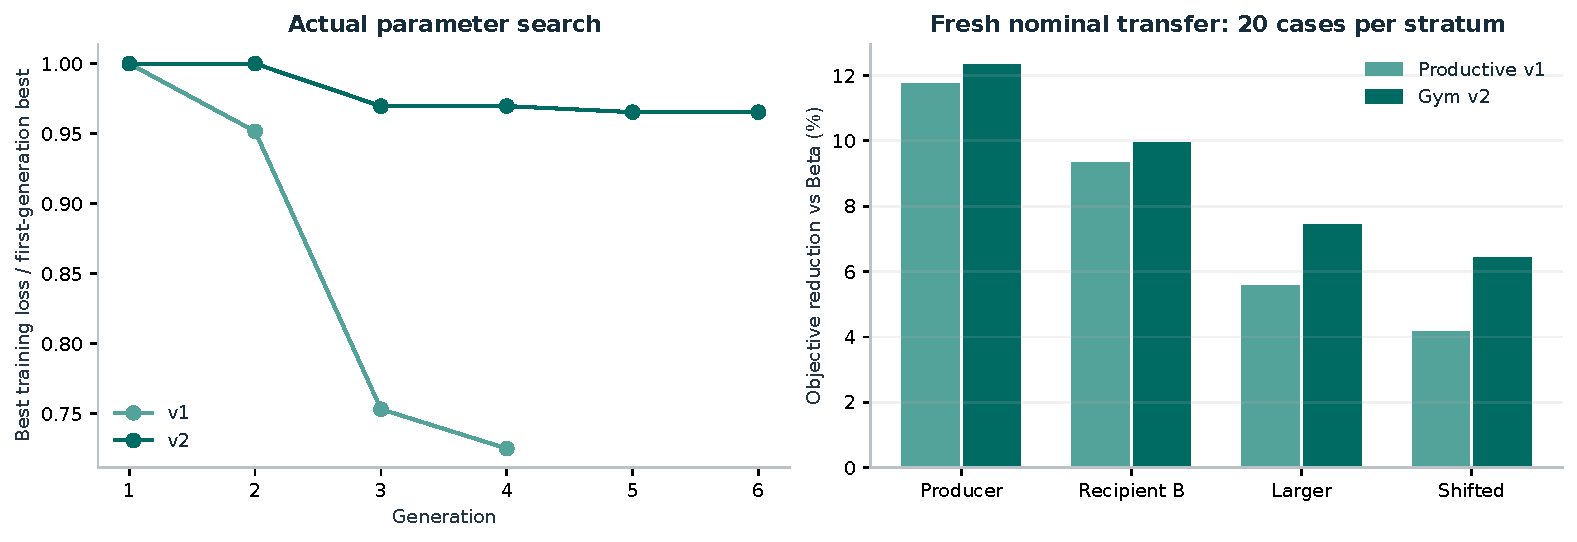
\includegraphics[width=\linewidth]{figures/learning-transfer.pdf}
\caption{Actual learning and fresh transfer. Left: each campaign's best training loss is normalized to its own first-generation best; v1 and v2 therefore are not compared as if they trained on identical tasks. Right: fixed-budget nominal gains on four fresh strata. The recipient stratum changes the number of jobs, machines and weight distribution.}
\label{fig:learning}
\end{figure}

The recipient stratum is particularly relevant to network transfer. Its twenty 40-job, four-machine confirmation instances are absent from training, although the Gym includes other instances from this stratum. Reloading v2 produces a mean objective reduction of 9.96\% versus the competent portfolio on those cases. Figure~\ref{fig:schedules} shows two delivered schedules for the first preselected recipient case. This is transfer of a compatible executable parameter policy. It is not evidence that a natural-language summary preserves expertise or that the recipient acquires another agent's general intelligence.

\begin{figure}[htbp]
\centering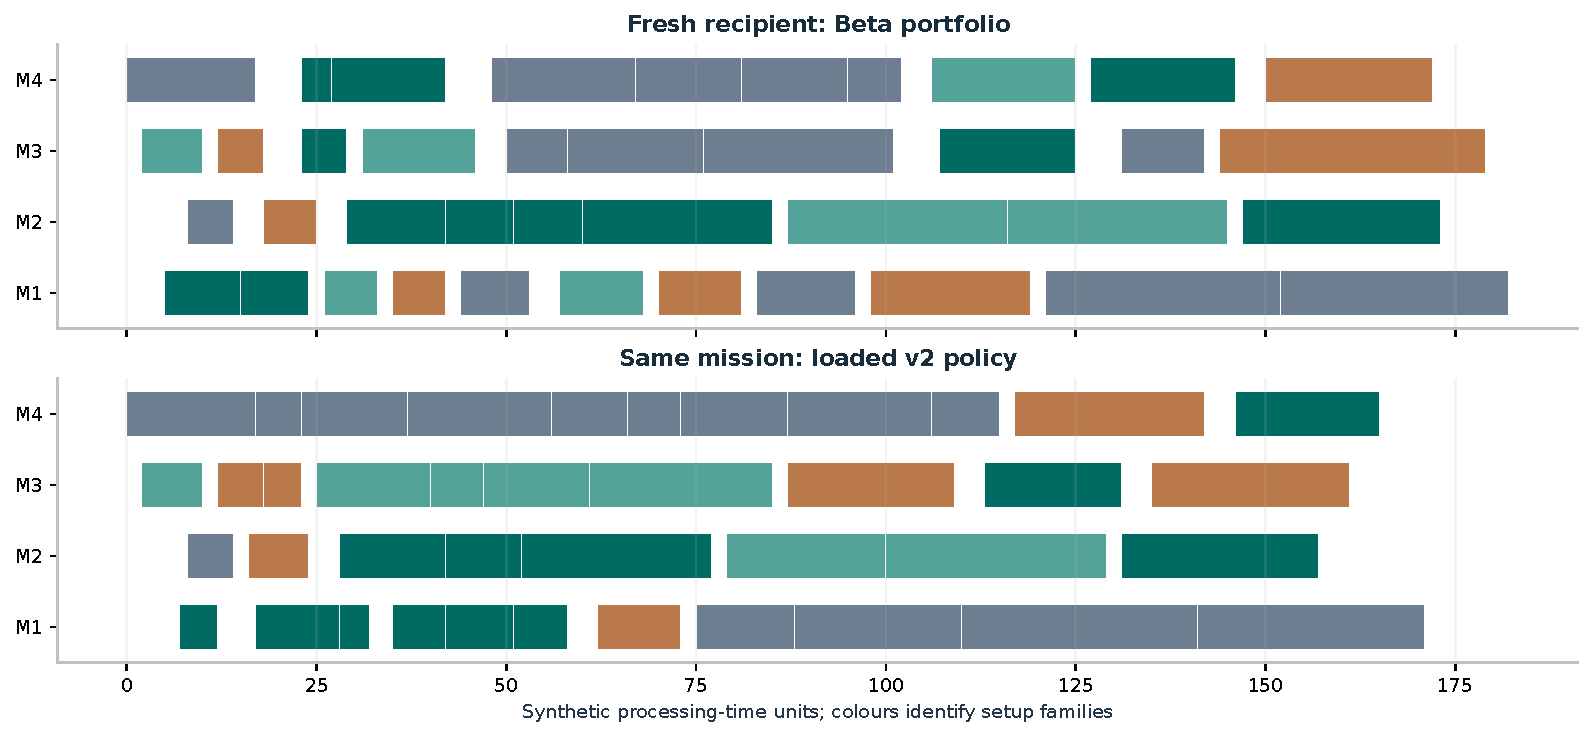
\includegraphics[width=\linewidth]{figures/delivered-schedules.pdf}
\caption{A concrete fresh recipient deliverable, case \texttt{recipient-51001}. Colours identify job families, which determine setup requirements. Both schedules preserve all jobs and all machine, release and setup constraints. The policy changes assignment and sequence; it does not change the acceptance checker or delete difficult work. Full input, schedule and verifier records are retained.}
\label{fig:schedules}
\end{figure}

\subsection{What the ablations identify, and what they do not}

The reversed-weight control has the same learned coefficients in the wrong feature positions. It still improves the nominal objective by about 2.36\% versus Beta because inserting another candidate also changes the search trajectory. The direct learned-v2 versus reversed-weight contrast is 6.58\% (4.92--8.19\%). This distinguishes much of the learned parameter content from the mere presence of an extra search starting point, without claiming that reversal is a competitive operating policy.

\begin{figure}[htbp]
\centering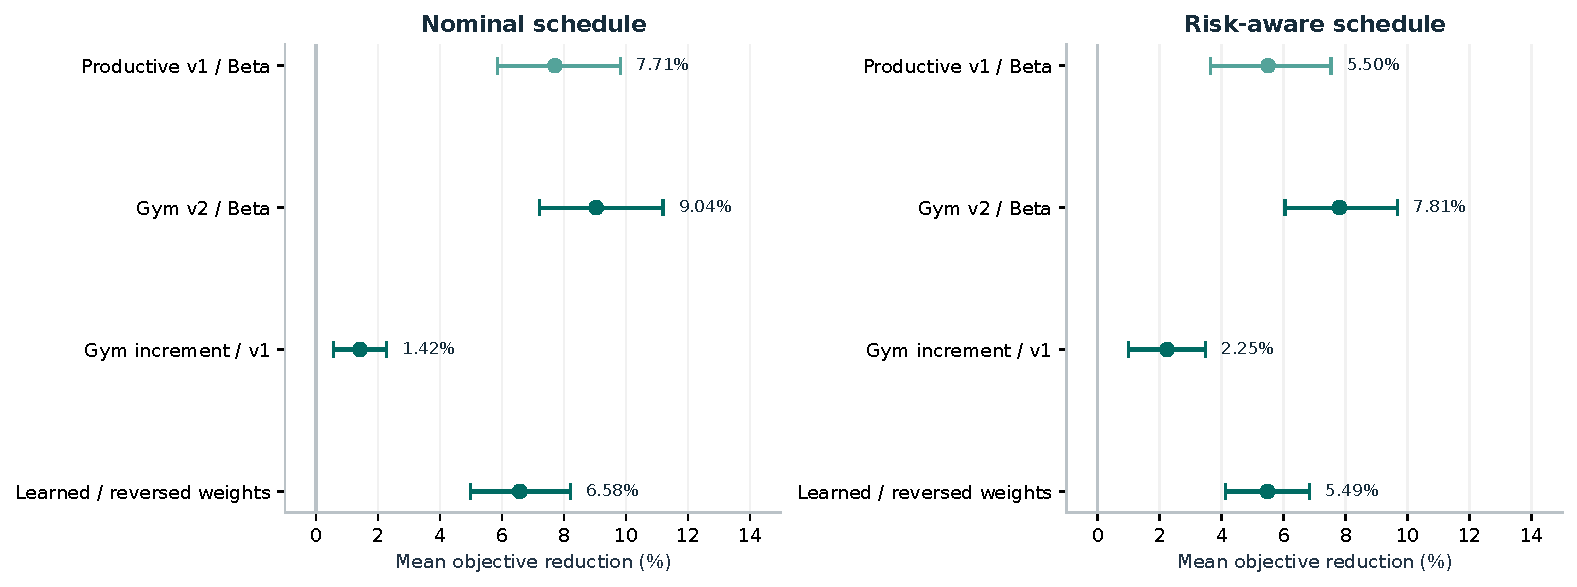
\includegraphics[width=\linewidth]{figures/causal-comparisons.pdf}
\caption{Paired objective reductions, with bootstrap intervals over the 80 fresh cases. For robust comparisons, ``Gym v2'' means v2 combined with the same scenario-ranking component used by the other fair robust arms. Intervals describe the sampled synthetic task distribution and are not evidence of external industrial generalization.}
\label{fig:causal}
\end{figure}

Composed v2 reduces the robust objective by 7.81\% (6.00--9.69\%) versus risk-aware Beta. The matched comparison to v1 with the same risk evaluator yields an incremental Gym effect of 2.25\% (1.06--3.49\%). These are interpretable policy improvements under equal candidate and scenario budgets.

The isolated risk-ranking ablation is weaker. Adding scenario ranking to v2 yields only 0.59\% mean improvement, with an interval from $-0.55$ to 1.75\%, and consumes additional scenario computation relative to the removal arm. This comparison neither convincingly establishes a positive isolated effect nor holds resources constant. The robust service also exists for Beta. Consequently, the lineage demonstrates compatible composition and useful robust schedules, but it does not establish that specialist synergy created an otherwise infeasible offering.

\subsection{A more demanding quality frontier is visible}

The primary acceptance standards remain unchanged. A secondary grid of improvement targets, frozen before the numerical investigator inspected confirmation outcomes, examines 0, 5, 10, 15, 20, 30 and 40\% reductions from the same incumbent. Every grid point is reported. At the 30\% tier, nominal acceptance is 49/80 for Beta, 63/80 for v1 and 67/80 for v2. Robust acceptance is 50/80 for Beta and 67/80 for both v1 and composed v2. This is evidence of expanded \emph{technical} delivery at a specified quality threshold, not demand for a premium product.

\begin{figure}[htbp]
\centering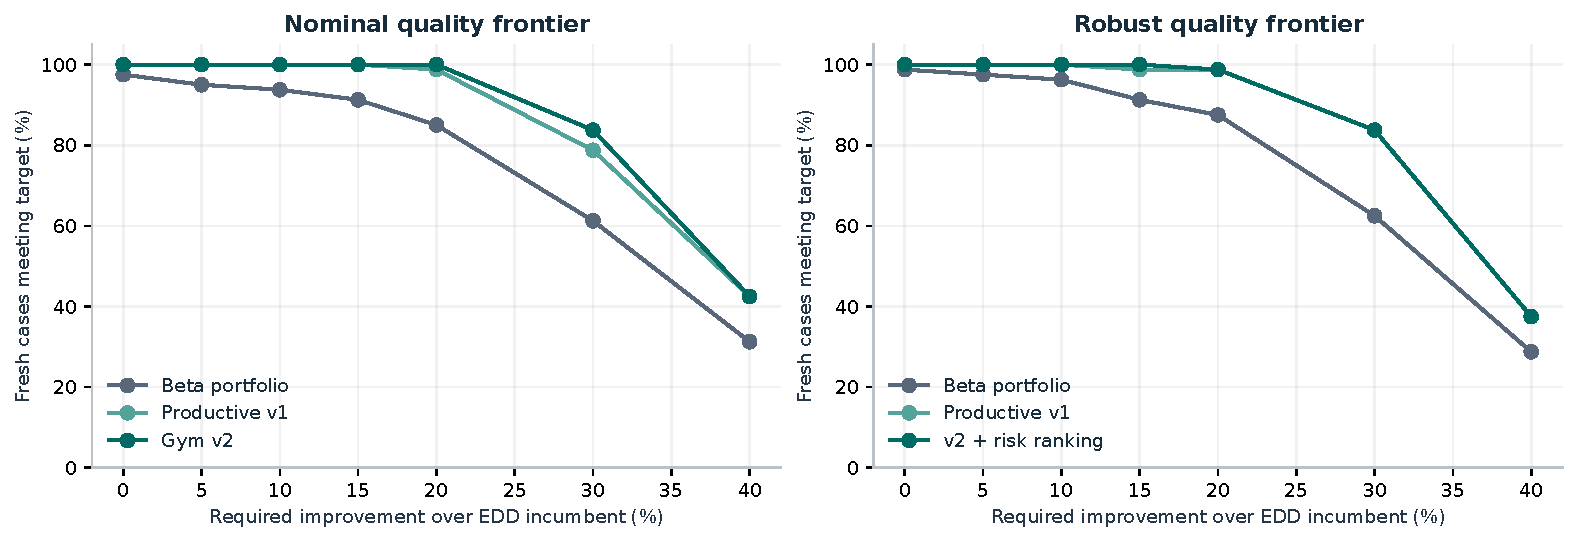
\includegraphics[width=\linewidth]{figures/quality-frontier.pdf}
\caption{Secondary quality frontier, preserving the original hard constraints and incumbent. A stricter contract admits fewer outcomes. Learned policies enlarge the set in parts of this finite grid. A stricter numerical contract is not automatically a more valuable customer product. The zero-improvement tier is also sensitive to a competent incumbent fallback.}
\label{fig:quality}
\end{figure}

\subsection{A conventional alternative catches up}

The expanded classical parameter grid at the same 48-candidate budget is worse on average. It is preserved as an unsuccessful baseline modification; it cannot be advertised as a stronger successor. A more consequential alternative simply increases the unchanged generic search budget to 144 candidates. An initial diagnostic on twelve preselected cases suggested catch-up. We then froze a separate addendum and evaluated twelve new cases, with no retraining or policy selection and with all three methods run on the same inputs.

\begin{table}[htbp]
\centering\small
\begin{tabular}{lrr}
\toprule
New twelve-case confirmation & Nominal & Robust\\
\midrule
Beta144 improvement over Beta48 & 4.49\% & 6.27\%\\
Learned48 improvement over Beta48 & 3.18\% & 4.31\%\\
Learned48 improvement over Beta144 & $-1.42$\% & $-2.10$\%\\
Primary acceptance, each method & 12/12 & 12/12\\
30\% tier: Beta48 / learned48 / Beta144 & 9 / 10 / 11 & 8 / 10 / 11\\
Mean solve seconds, Beta48 & 0.155 & 0.176\\
Mean solve seconds, learned48 & 0.149 & 0.171\\
Mean solve seconds, Beta144 & 0.464 & 0.515\\
\bottomrule
\end{tabular}
\caption{Fresh stronger-search sensitivity. Beta144 uses three times the candidate budget, so this is not a fixed-resource reversal of the primary experiment. It is an operating alternative whose extra resources must be priced. Twelve cases provide limited population evidence.}
\label{tab:catchup}
\end{table}

The learned advantage over Beta144 has an interval of $-4.93$ to 2.24\% for nominal work and $-4.10$ to approximately zero for robust work. The robust upper endpoint is slightly below zero, but the sample is small and intervals are unadjusted. A broad superiority claim would be unwarranted. The practical observation is that extra generic search is inexpensive: using an explicitly assumed \USD3 per CPU-hour rate and elapsed solver time as a compute-cost proxy, its incremental cost is roughly \USD0.00026--0.00028 per job. The entire v2 numerical search is also inexpensive, taking roughly six measured seconds in the primary run. Any much larger Gym bill therefore represents assumed integration, orchestration, assessment or upkeep, rather than measured numerical training expense.

OR-Tools CP-SAT supplies a separate formulation check. Twelve instances and two warm starts were evaluated at 0.08 and, in a preserved extension, 1.0 deterministic-time units. All calls returned feasible schedules but did not improve their supplied warm starts, and their bounds remain wide. This outcome validates a finite solver interface but leaves the optimization challenge unresolved within those budgets; it does not establish superiority over a well-tuned industrial solver. The primary Beta remains a bounded algorithmic proxy, not the ceiling of current frontier reasoning equipped with suitable tools.

\section{Commercial consequences under declared assumptions}
\label{sec:economic-results}

\subsection{Profitable production and new-offering value are separable from Alpha}

The simulator runs 128 matched worlds per scenario and policy. It prices an initial bounded schedule package against an estimated \CAD3,220 human-service reference and a broader risk-aware package against \CAD7,217. These references use sourced professional rate categories and researcher-estimated hours; they are not quoted sales. The assumed CAD-to-USD conversion is 0.73, not a claim about the spot exchange rate. Prices are searched over 0.35--1.10 times the reference. The search can reach a boundary, and the finite choice is not a globally optimal or market-validated quote.

\begin{table}[htbp]
\centering\small
\begin{tabular}{lrrrr}
\toprule
Central assumptions & Collections & Expenses & Accrued profit & Available funds\\
\midrule
\EconomicRows
\bottomrule
\end{tabular}
\caption{Mean 90-day modeled accounts, USD, over 128 matched histories. Accrued profit includes accepted-work receivables; collections do not. Available funds are cash after reserve and obligations and include remaining seed capital. These values are conditional simulation outputs, not a forecast, earned revenue or customer validation. All policies start with the same \USD8,000 and four modeled production-capacity hours per day.}
\label{tab:economics}
\end{table}

Under central assumptions, Beta's initial offering earns about \USD114,859 modeled accrued profit. The shared enterprise allowed to launch the adjacent offering reaches about \USD218,054. That contrast could easily be misread as a dramatic learning flywheel. The equal-menu control resolves it: Beta allowed to launch the same offering reaches about \USD215,842. The matched incremental program contribution is approximately \USD2,212, far smaller than the gross menu-expansion contrast. The opportunity itself, assumed demand and pricing account for most of the modeled difference. The best initial policy can therefore be profitable production with ordinary tools.

The controller does not force training. In central worlds, the opportunity policy attempts retention in about 66.4\% of histories and Gym in only 2.3\%; it does not choose the composition campaign. Development acceptance was 24/24 across methods, so a controller with honest information could not initially foresee the later Beta failures. It learns through subsequent observations. An analyst who inserted fresh confirmation success rates into its initial beliefs would give it information it did not possess.

\begin{figure}[htbp]
\centering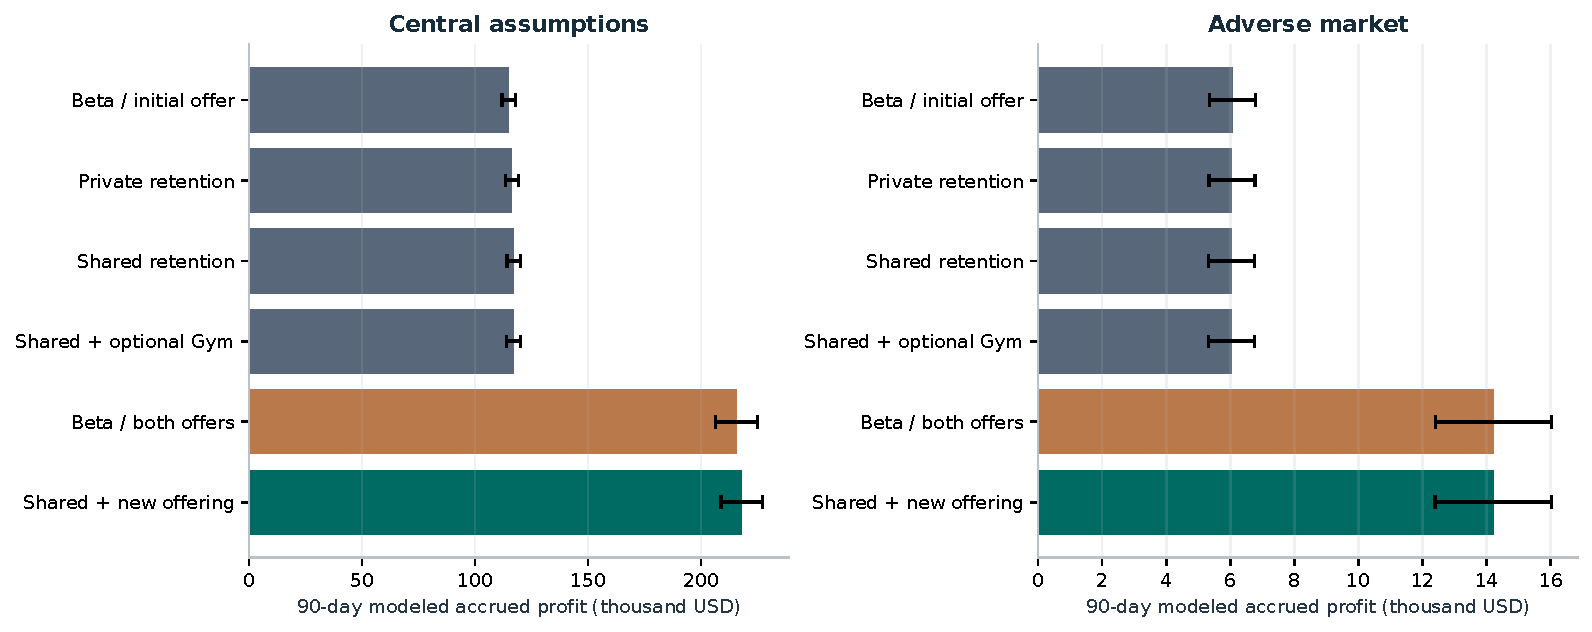
\includegraphics[width=\linewidth]{figures/enterprise-comparisons.pdf}
\caption{Matched commercial comparisons under two sets of unsupported market assumptions. Error bars describe Monte Carlo uncertainty conditional on those assumptions. Equal-menu Beta is essential: comparing only the first and last policy would attribute much of a larger product menu's value to learning.}
\label{fig:enterprise}
\end{figure}

Thin demand changes the decision. Initial-offer Beta earns about \USD4,313 on average, with a 20.3\% simulated loss frequency. All retention policies decline learning and coincide. The two-offer policies can still show positive modeled contribution, but Beta and the shared enterprise coincide there too. Under the adverse-market scenario, the shared opportunity policy's incremental contribution relative to equal-menu Beta is slightly negative. Faster obsolescence and fragile transfer sharply reduce the incremental gain. These are counterexamples to mandatory reinvestment or an automatic network premium.

\subsection{Demand, costs and quality bound investment value}

Figure~\ref{fig:commercial} sweeps qualified-lead arrival and marginal delivery/R\&D cost for equal-menu Beta and the shared opportunity policy. It is a conditional profit sensitivity, not a located absolute enterprise break-even boundary. Every displayed grid-cell mean remains positive; the minimum is about \USD2,546, while the minimum across the seven primary scenarios and eleven policies is about \USD4,313. Individual simulated worlds can still lose money. These ranges identify changes in profit and in the incremental value of learning, but do not locate where mean enterprise profit reaches zero along demand or cost. Higher arrival rates eventually meet the fixed daily capacity. The separate expansion policy must finance its extra capacity with collected cash above original capital and reserve; its results cannot be pooled with fixed-resource comparisons as evidence of a network effect.

\begin{figure}[htbp]
\centering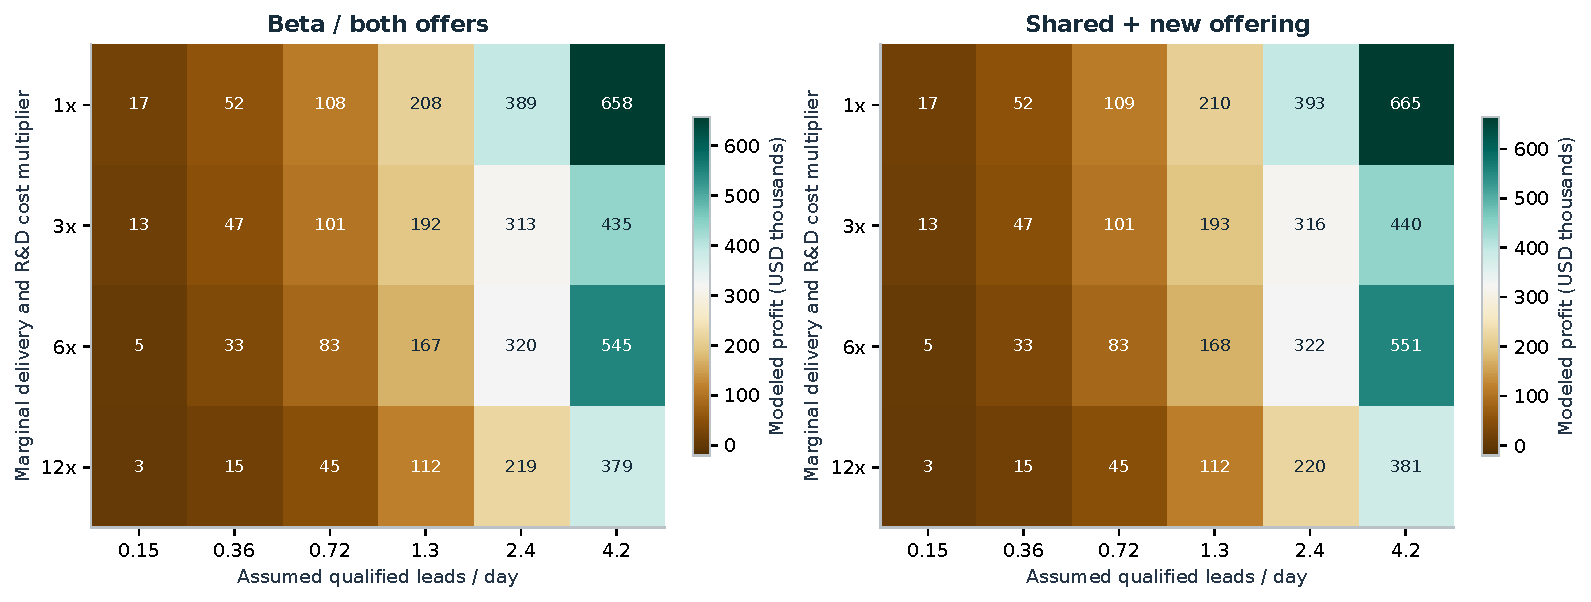
\includegraphics[width=\linewidth]{figures/commercial-frontier.pdf}
\caption{Conditional 90-day profit sensitivity. Each cell is the mean of matched simulated histories, in USD thousands. All displayed means are positive, so this demand--cost grid does not identify an absolute enterprise break-even boundary. Market arrival, price response and cost envelopes remain assumptions; these values do not demonstrate attainable revenue.}
\label{fig:commercial}
\end{figure}

The secondary quality-contract analysis preserves every target and repeats matched enterprise decisions with development-only priors. Under the central market, the shared opportunity policy's incremental profit over equal-menu Beta rises from roughly \USD565 at the zero-improvement tier to a grid maximum near \USD12,705 at 20\%, then \USD12,548 at 30\% and about \USD2,113 at 40\%. It is not monotonic. These are different hypothetical contracts, not permission to substitute a favorable threshold for the primary result. Under thin demand, learning-program increments are zero throughout the grid because the controller does not invest.

Absolute losses do appear in that separate stricter-contract sensitivity. With the executed portfolio and thin demand, initial-offer Beta's mean accrued profit falls from about \USD2,646 at the 20\% contract to negative \USD1,455 at 30\% and negative \USD3,502 at 40\%; the latter loses money in 92.2\% of simulated worlds. This brackets a conditional sign change between two tested quality requirements for one policy and assumed market. It does not locate a continuous break-even threshold or establish the boundary for the best available policy. The distinction matters: declining optional learning can be rational even when the remaining business is itself unprofitable.

A hypothetical future Beta that attains the best available per-case capability removes the program increment through the 30\% tier; the remaining 40\% increment is small with an interval spanning zero. That hypothetical envelope is not a live model result and gives no policy access to future outcomes. It changes the modeled external capability distribution, with matching development priors, to ask whether retained value survives frontier catch-up. The independently executed Beta144 addendum provides a concrete, smaller-scale reason to take this sensitivity seriously.

The identical-content ordinary library and graph-labeled policy produce identical results. No graph-specific value is encoded or observed. Provenance links help inspection, but they are not automatically a productivity multiplier. Likewise, synthetic cryptographic admission and numerical superiority do not establish customer value. The business effect must pass through useful accepted work, actual collections and a complete account.

\subsection{Measured compute and assumed program overhead must not be conflated}

The primary program envelopes are \USD120 for retention, \USD90 for sharing, \USD420 for optional Gym, and \USD180 for composition. New-offering development and independent assessment are modeled separately at \USD850 and \USD150. These are declared assumptions. They are not API invoices, measured human work or the cost of six seconds of CEM computation. The companion reports lower automated program envelopes and the measured numerical floor separately. A floor omitting qualification and maintenance is not a complete operating cost; an arbitrary expensive program is not evidence that economical training fails.

The twelve-case stronger-Beta addendum makes this distinction concrete. At the secondary 30\% quality contract, the learned method adds conditional contribution of about \USD144 per booked nominal job and \USD643 per robust job relative to Beta48. Including two maintenance cycles, the primary additional program envelopes of \USD700 and \USD880 reach point-estimate break-even after five and two uses. Against Beta144, the same learned method instead loses about \USD144 and \USD322 per job at this tier. Reducing training expense cannot repair a negative operating contribution. This is not universal dominance: at the 40\% robust tier the learned policy passes 3/12 and Beta144 2/12. All tiers and wide paired-case intervals remain in the companion. Common launch and automation expenses cancel in these matched per-booked-job contrasts; they remain charged in the full enterprise accounts.

\begin{figure}[htbp]
\centering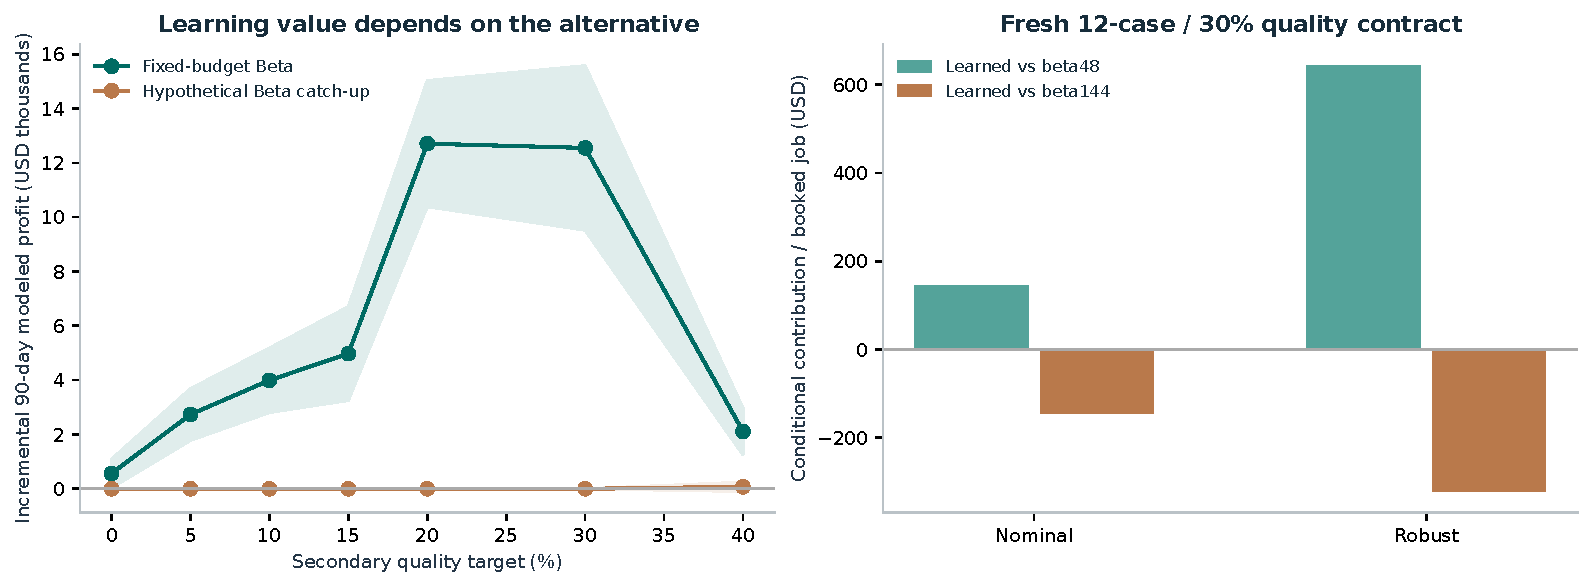
\includegraphics[width=\linewidth]{figures/investment-boundary.pdf}
\caption{Where an optional learning program can be worthwhile. Left: the conditional 90-day increment over equal-menu Beta changes with contract difficulty and disappears under a hypothetical best-capability Beta envelope. Shading is conditional Monte Carlo uncertainty. Right: in the independent twelve-case addendum, the same learned method has positive point-estimate contribution against Beta48 and negative contribution against Beta144 at the 30\% tier. The latter has three times the candidate budget. These are small-sample conditional economics, not customer observations.}
\end{figure}

The economically relevant decision is comparative. For an anticipated number $N$ of eligible future uses, a capability is worthwhile only if its expected incremental collected contribution, after incremental serving and maintenance, exceeds additional assessment and development expense plus the value of displaced work. We keep the displacement term in the decision score rather than subtracting it again from a cash account that already records lost production. When a credible ordinary alternative delivers comparable quality for a fraction of a cent of additional compute, the retained program must justify itself through stronger quality, reliability, workload scale or a different opportunity. The present evidence does not establish that justification universally.

\section{Transformational intelligence: three audited attempts}

Transformational intelligence is operational here as a recorded attempt to change how a purpose is achieved. It is not an honorific assigned after a score rises. Table~\ref{tab:transformations} separates the proposal, discriminating experiment and supported consequence.

\begin{table}[htbp]
\centering\small
\begin{tabularx}{\linewidth}{L{0.17\linewidth}YYY}
\toprule
Purpose and obstacle & Proposed change & Discriminating evidence & Consequence\\
\midrule
Better schedules under finite search & Retain seven dispatch weights learned across productive work & Same tasks, hard constraints and 48 candidates; fresh recipient and reversed-weight control & Transferable fixed-budget advantage; generic extra search can catch up\\
Reliable planning with uncertain durations & Combine dispatch and empirical uncertainty replay & Fresh disturbance evaluation; same risk component available to Beta; ranking-removal ablation & Useful robust schedules; isolated composition benefit remains inconclusive\\
Choose a worthwhile next service & Jointly price, select work and consider risk-aware offering & Matched opportunities; equal-menu Beta and private controls; complete cost and downside & Conditional expansion value; most is not uniquely attributable to Alpha\\
\bottomrule
\end{tabularx}
\caption{Transformation records preserve purpose and evaluator. The alternative is allowed to fail. These are bounded strategy and workflow changes, not evidence of autonomous invention of new laws, models or markets.}
\label{tab:transformations}
\end{table}

The principal failed hypothesis is instructive: a capability improving existing work need not create a new product that ordinary methods cannot deliver. We did not repair this failure by granting only the shared policy access to the robust customer application. Instead, that access was supplied to competent controls. A future stronger result would need a real constraint that the specialized combination satisfies and the best economically available general alternative does not, followed by independent buyer evidence that the constraint matters.

\section{Operating blueprint supported by this edition}

\subsection{Start with a bounded, auditable planning package}

The candidate initial offering is a manufacturing schedule-design package for a planner who can supply validated processing-time estimates, release times, due dates, job priorities, machine eligibility and setup relationships. The demonstrated computational scope is 32--64 jobs on three or four machines. The deliverable should include the full schedule, an independent feasibility report, comparison with the buyer's approved incumbent, assumptions, a reproducible input snapshot and failure conditions. The buyer approves the objective and acceptance rule before work begins. A plant deployment, enterprise-resource-planning integration, safety-critical machine instruction, labor-law schedule or rolling breakdown-recovery service is outside this edition's evidence.

The modeled package requires customer data preparation and signoff. The local solver is fast, but the complete intake, missing-data resolution, packaging, contractual turnaround and operating capacity have not been measured in a customer trial. The operator should sell a bounded decision artifact with an agreed delivery window, then measure the whole process. The source-backed human reference is a transparent benchmark for testing prices, not proof that an automated offer can command it.

\subsection{Use ordinary search as a live alternative in every decision}

Begin qualification with a competent generic portfolio and a suitable constraint solver. Keep the buyer's incumbent as a safe reference and retain the option of additional ordinary search. The fixed-budget learned policy is a promising candidate, not a compulsory production dependency. Retain it only when fresh local evidence, rights and compatible execution establish useful incremental value. Store the executable parameters and compatible implementation, not only a textual explanation. Recheck applicability when eligibility, setups, objective weights, uncertainty or customer requirements change.

Consider Gym practice when the remaining quality gap matters to a buyer and an economical development experiment can resolve it. Charge the extra work once in C and any additional independent assessment in B. Stop if expanded ordinary search, a solver upgrade, low demand or impending obsolescence makes the experiment's expected value negative. The primary result already shows that most of the nominal gain is present in productive v1; there is no evidence-based reason to require v2 before selling useful work.

\subsection{Share only the artifact and authority actually qualified}

The demonstrated sharing form is a compatible executable parameter policy. The study does not train or distribute a proprietary checkpoint. An authenticated specialist service would be a different delivery form with its own custody, reliability, latency and invocation costs; invoking such a service would not mean the recipient independently owns its intelligence. Each version requires scope, dependencies, license, provenance, evidence, resource requirements, revocation and failure limits.

The current protected runtime correctly rejects arbitrary scheduling-capsule admission. The actual native controls exercise two synthetic RPC readers, two synthetic agent identities, real signature verification and refusal of unauthorized, repeated and revoked requests. They do not make the scheduling policy available to live \texttt{*.agent.agi.eth} members. Production availability must follow the existing runtime owner's qualified extension and the existing ENS, Jobs validator, governance and settlement boundaries. The study does not create another production registry or publisher.

\subsection{Test the next offering through a buyer, not through a label}

The adjacent candidate is a risk-aware schedule and scenario dossier for a planner whose late-work exposure is sensitive to uncertain durations. A credible pilot would establish the customer's historical disturbance distribution, compare the actual generic and specialized alternatives under the same delivery budget, specify what uncertainty statements the buyer needs, and collect a real willingness-to-pay decision. If Beta can deliver the same valued outcome more cheaply, launch with Beta. If the customer does not value the extra dossier, defer it. An offered business concept and a simulated collection are not sales.

\begin{findingbox}
\textbf{Next live qualification gate.} Obtain rights-cleared customer inputs and a prespecified acceptance contract; measure the complete generic and retained-policy workflows; validate the runtime's scientific capability scope and current identity authority; document observed acquisition, correction and support costs; and run a paid pilot with actual collection evidence. No commercial or specialist-ASI claim should advance beyond the evidence produced by that gate.
\end{findingbox}

\section{Conclusion}

Productive activity can leave behind a useful executable specialist in this bounded domain. The learned artifact transfers to fresh recipients and improves more demanding schedules. Optional Gym practice adds a smaller measurable improvement. Those findings survive direct artifact inspection and matched computational comparisons.

The economic conclusion is narrower and more useful than an automatic flywheel claim. Profitable delivery can exist without retention. A new offering can be worthwhile without being created by the specialist. Additional generic search can remove the advantage that appeared valuable at a smaller fixed budget. The best enterprise policy is therefore conditional: deliver, learn, share, combine, expand, preserve cash or stop according to the best currently supported alternative. An enterprise that can reject its own proposed advantage is closer to the requested mechanism than one required to report compounding.

\clearpage
\appendix
\section{Evidence classes, custody and reproduction}

\begin{longtable}{L{0.19\linewidth}L{0.34\linewidth}L{0.39\linewidth}}
\toprule
Evidence class & Examples in this edition & Permitted interpretation\\
\midrule\endhead
Observed execution & CEM parameter updates, candidate traces, valid schedules, fresh objectives, native signatures, accounting replay & These programs ran on the recorded finite inputs; the source and results can be inspected and replayed\\
Sourced & Official model identifiers and prices; AFG professional rate categories; first-party consulting offer & Documentation or market-category evidence at the retrieval date, not account access or matched sales\\
Derived/calibrated & Technical success and quality distributions from development and confirmation records & A finite empirical input to the conditional model; no general frontier-model calibration\\
Assumed & Scope hours, conversion, demand, model-token volumes, residual exceptions, program cost, currency conversion & Exposed scenario inputs requiring measurement for live qualification\\
Simulated & Buyers, campaigns in enterprise worlds, collections, profit, synthetic ENS readers and labels & Conditional behavior; no actual customer, revenue or live namespace access\\
Not established & Autonomous discovery, unique product creation through composition, current frontier superiority, sustained compounding, specialist ASI & Remains outside the supported claims\\
\bottomrule
\end{longtable}

The primary source is frozen at repository commit \texttt{80b345828f34fd8a6e592977dd17ef37141305f4}. Eighteen unchanged runtime files are included in a source-pinned reproduction snapshot, with their original license and byte hashes. New work is isolated under \texttt{studies/agi-alpha-next-advantage-v1/}. Existing papers and demonstrations are preserved. The source map records parallel owners and unavailable original materials. The active v1.46 publication lease is respected; a review artifact is not a release-qualified public deployment.

The evidence manifest binds code, configurations, raw records, policies, figures, manuscript and browser edition. Its own hash is excluded to avoid a circular identity. Numerical source freezes predate primary confirmation. The first interrupted numerical attempt is retained separately: a provenance and latent-parameter isolation repair triggered fresh confirmation seeds, without using the interrupted outcomes for tuning. The original cash-only expansion run is also retained separately because its funding boundary did not establish earned-surplus financing. No failed source is silently reclassified as qualified.

\subsection{Reproduction entry points}

The complete command sequence, exact direct dependency versions and environment limits are in \texttt{REPRODUCE.md}. Work in a disposable copy to preserve original bytes and timing records. The minimal computational entry points are:
\begin{quote}\small\ttfamily
python src/numerical.py\\
python evidence/numerical/quality\_frontier\_analysis.py\\
python evidence/numerical/beta144\_confirmation.py\\
python src/economics.py\\
python src/replay\_expansion.py --output /tmp/expansion-replay\\
python src/build\_report.py\\
python web/build\_web.py --strict\\
cd paper \&\& latexmk -pdf -interaction=nonstopmode enterprise-next-advantage.tex
\end{quote}
The native accounting adapter takes the representative simulated expense events and collections and replays them through the preserved journal and ledger. Its report must match collection-based cash profit, not the simulator's accrual profit. Numerical times and signatures can vary between executions; those differences must not be normalized into a false byte-for-byte reproduction claim. Original evidence and a new execution should remain separate.

The final local study suite passes 44 directed tests. The representative native replay binds 449 economic events into 68 verified signed journal events and reconciles \USD144,796.96 collections, \USD14,297.50 complete expenses, \USD130,499.46 collection-based profit and \USD136,699.46 available funds. These are simulated money amounts processed by actual accounting software. The separate accrual profit is \USD140,842.10 because \USD10,342.64 remains receivable. These local tests do not replace the repository's configured hosted review, full release qualification or public served-byte checks.

\subsection{Finite budgets and remaining uncertainty}

The corrected main numerical experiment retains 64,064 schedule evaluations and 599,040 selection-scenario evaluations. The interrupted attempt retains at least 20,672 schedule evaluations and 172,800 scenario evaluations. The final stronger-Beta confirmation adds 17,280 schedule evaluations and 207,360 scenario evaluations; separate CP-SAT extensions have their own logs. These counts are research-execution resources, not automatically charges to each hypothetical enterprise. Researcher labor, compilation, process startup, I/O and any unsaved interrupted computation were not completely measured and must not be described as zero.

The simulation's 128 histories are repeated stochastic business worlds over a fixed technical case pool. They do not constitute 128 new numerical trials or a survey of customers. The supplementary quality study likewise does not create new technical evidence by resampling the same cases. Multiple unadjusted numerical comparisons, a small stronger-Beta confirmation, public generator seeds and same-session verification limit confirmatory strength. A genuinely protected independent replication and a live customer study remain necessary for stronger external claims.

\bibliographystyle{unsrtnat}
\bibliography{references}
\end{document}
